% Options for packages loaded elsewhere
\PassOptionsToPackage{unicode}{hyperref}
\PassOptionsToPackage{hyphens}{url}
%
\documentclass[
]{article}
\title{P2}
\author{Tobias Pedersen, Dat Luong, Adam Rumi, Kristoffer Lading,
Xiaoyin Chang, Kasper Sommer}
\date{4/3/2022}

\usepackage{amsmath,amssymb}
\usepackage{lmodern}
\usepackage{iftex}
\ifPDFTeX
  \usepackage[T1]{fontenc}
  \usepackage[utf8]{inputenc}
  \usepackage{textcomp} % provide euro and other symbols
\else % if luatex or xetex
  \usepackage{unicode-math}
  \defaultfontfeatures{Scale=MatchLowercase}
  \defaultfontfeatures[\rmfamily]{Ligatures=TeX,Scale=1}
\fi
% Use upquote if available, for straight quotes in verbatim environments
\IfFileExists{upquote.sty}{\usepackage{upquote}}{}
\IfFileExists{microtype.sty}{% use microtype if available
  \usepackage[]{microtype}
  \UseMicrotypeSet[protrusion]{basicmath} % disable protrusion for tt fonts
}{}
\makeatletter
\@ifundefined{KOMAClassName}{% if non-KOMA class
  \IfFileExists{parskip.sty}{%
    \usepackage{parskip}
  }{% else
    \setlength{\parindent}{0pt}
    \setlength{\parskip}{6pt plus 2pt minus 1pt}}
}{% if KOMA class
  \KOMAoptions{parskip=half}}
\makeatother
\usepackage{xcolor}
\IfFileExists{xurl.sty}{\usepackage{xurl}}{} % add URL line breaks if available
\IfFileExists{bookmark.sty}{\usepackage{bookmark}}{\usepackage{hyperref}}
\hypersetup{
  pdftitle={P2},
  pdfauthor={Tobias Pedersen, Dat Luong, Adam Rumi, Kristoffer Lading, Xiaoyin Chang, Kasper Sommer},
  hidelinks,
  pdfcreator={LaTeX via pandoc}}
\urlstyle{same} % disable monospaced font for URLs
\usepackage[margin=1in]{geometry}
\usepackage{color}
\usepackage{fancyvrb}
\newcommand{\VerbBar}{|}
\newcommand{\VERB}{\Verb[commandchars=\\\{\}]}
\DefineVerbatimEnvironment{Highlighting}{Verbatim}{commandchars=\\\{\}}
% Add ',fontsize=\small' for more characters per line
\usepackage{framed}
\definecolor{shadecolor}{RGB}{248,248,248}
\newenvironment{Shaded}{\begin{snugshade}}{\end{snugshade}}
\newcommand{\AlertTok}[1]{\textcolor[rgb]{0.94,0.16,0.16}{#1}}
\newcommand{\AnnotationTok}[1]{\textcolor[rgb]{0.56,0.35,0.01}{\textbf{\textit{#1}}}}
\newcommand{\AttributeTok}[1]{\textcolor[rgb]{0.77,0.63,0.00}{#1}}
\newcommand{\BaseNTok}[1]{\textcolor[rgb]{0.00,0.00,0.81}{#1}}
\newcommand{\BuiltInTok}[1]{#1}
\newcommand{\CharTok}[1]{\textcolor[rgb]{0.31,0.60,0.02}{#1}}
\newcommand{\CommentTok}[1]{\textcolor[rgb]{0.56,0.35,0.01}{\textit{#1}}}
\newcommand{\CommentVarTok}[1]{\textcolor[rgb]{0.56,0.35,0.01}{\textbf{\textit{#1}}}}
\newcommand{\ConstantTok}[1]{\textcolor[rgb]{0.00,0.00,0.00}{#1}}
\newcommand{\ControlFlowTok}[1]{\textcolor[rgb]{0.13,0.29,0.53}{\textbf{#1}}}
\newcommand{\DataTypeTok}[1]{\textcolor[rgb]{0.13,0.29,0.53}{#1}}
\newcommand{\DecValTok}[1]{\textcolor[rgb]{0.00,0.00,0.81}{#1}}
\newcommand{\DocumentationTok}[1]{\textcolor[rgb]{0.56,0.35,0.01}{\textbf{\textit{#1}}}}
\newcommand{\ErrorTok}[1]{\textcolor[rgb]{0.64,0.00,0.00}{\textbf{#1}}}
\newcommand{\ExtensionTok}[1]{#1}
\newcommand{\FloatTok}[1]{\textcolor[rgb]{0.00,0.00,0.81}{#1}}
\newcommand{\FunctionTok}[1]{\textcolor[rgb]{0.00,0.00,0.00}{#1}}
\newcommand{\ImportTok}[1]{#1}
\newcommand{\InformationTok}[1]{\textcolor[rgb]{0.56,0.35,0.01}{\textbf{\textit{#1}}}}
\newcommand{\KeywordTok}[1]{\textcolor[rgb]{0.13,0.29,0.53}{\textbf{#1}}}
\newcommand{\NormalTok}[1]{#1}
\newcommand{\OperatorTok}[1]{\textcolor[rgb]{0.81,0.36,0.00}{\textbf{#1}}}
\newcommand{\OtherTok}[1]{\textcolor[rgb]{0.56,0.35,0.01}{#1}}
\newcommand{\PreprocessorTok}[1]{\textcolor[rgb]{0.56,0.35,0.01}{\textit{#1}}}
\newcommand{\RegionMarkerTok}[1]{#1}
\newcommand{\SpecialCharTok}[1]{\textcolor[rgb]{0.00,0.00,0.00}{#1}}
\newcommand{\SpecialStringTok}[1]{\textcolor[rgb]{0.31,0.60,0.02}{#1}}
\newcommand{\StringTok}[1]{\textcolor[rgb]{0.31,0.60,0.02}{#1}}
\newcommand{\VariableTok}[1]{\textcolor[rgb]{0.00,0.00,0.00}{#1}}
\newcommand{\VerbatimStringTok}[1]{\textcolor[rgb]{0.31,0.60,0.02}{#1}}
\newcommand{\WarningTok}[1]{\textcolor[rgb]{0.56,0.35,0.01}{\textbf{\textit{#1}}}}
\usepackage{graphicx}
\makeatletter
\def\maxwidth{\ifdim\Gin@nat@width>\linewidth\linewidth\else\Gin@nat@width\fi}
\def\maxheight{\ifdim\Gin@nat@height>\textheight\textheight\else\Gin@nat@height\fi}
\makeatother
% Scale images if necessary, so that they will not overflow the page
% margins by default, and it is still possible to overwrite the defaults
% using explicit options in \includegraphics[width, height, ...]{}
\setkeys{Gin}{width=\maxwidth,height=\maxheight,keepaspectratio}
% Set default figure placement to htbp
\makeatletter
\def\fps@figure{htbp}
\makeatother
\setlength{\emergencystretch}{3em} % prevent overfull lines
\providecommand{\tightlist}{%
  \setlength{\itemsep}{0pt}\setlength{\parskip}{0pt}}
\setcounter{secnumdepth}{-\maxdimen} % remove section numbering
\ifLuaTeX
  \usepackage{selnolig}  % disable illegal ligatures
\fi

\begin{document}
\maketitle

\hypertarget{introduktion}{%
\section{Introduktion}\label{introduktion}}

I denne del af projektet, skabes der en Pseudo-Random Number generator,
hvis formål er at generere tilfældige tal. Fordelingen af disse tal vil
være uniform, og ved hjælp af en Box-Muller transformation vil der opnås
en normalfordeling. Grunden til dette er at undersøge stikprøver fra en
normalfordeling i forhold til Central Limit Theorem, da der er
adskillige interessante statistiske spørgsmål herinden under.

\hypertarget{pseudo-random-number-generators}{%
\section{Pseudo-Random Number
Generators}\label{pseudo-random-number-generators}}

For at kunne generere tilfældige tal ud fra deterministiske computere,er
det nødvendigt at bearbejde et input ved hjælp af en algoritme, således
at det genererede tal tilsyneladende er tilfældigt. Et sådanne genereret
tal kaldes et ``Pseudo-Random Number'', og disse bliver genereret ved
hjælp af Pseudo-Random Number Generators (også kaldet PRNG'er). PRNG'er
benytter et seed, som kan bestemmes af brugeren, til at generere de
tilfældige tal. Et eksempel på en kendt PRNG, er en Lineære Kongruentiel
Generator (Også kaldet LCG).

\hypertarget{true-random-number-generators}{%
\section{True-Random Number
Generators}\label{true-random-number-generators}}

I modsætning til PRNG'er, eksisterer der også True-Random Number
Generators (også kaldet TRNG'er). Disse generators genererer tilfældige
tal, uden nødvendigvis at afhænge af algoritmer. Et eksempel på en kendt
TRNG, er at generere tilfældige tal ved hjælp af atmosfærisk støj.

\hypertarget{sammenligning-af-prnger-og-trnger}{%
\section{Sammenligning af PRNG'er og
TRNG'er}\label{sammenligning-af-prnger-og-trnger}}

En PRNG er meget velegnet til simulationer, da det er muligt at
reproducere dataet ved at sætte seed'et til en bestemt værdi. Dette gør
det muligt for andre indenfor samme område, at kunne få dataet fra en
given simulation, og derved er det nemmere at diskutere fund og eller
problemer med den givne simulation.

TRNG'er kan også benyttes til simulationer, og siden tallene er mere
tilfældige i forhold til PRNG'erne, kan de være mere velegnet til
simulationer. Problemet er dog, at siden seedets værdi ikke kan
bestemme, er det umuligt at reproducere dataet. Grundet dette, er PRNG i
adskillige situationer foretrukket indenfor simulationer. Dog er det
værd at nævne, at siden dataet fra en TRNG ikke kan reproduceres, er det
optimalt for ting som skal være tilfældige, såsom lotteriet, gambling
eller kryptering.

I dette projekt vil en PRNG implementeres i R, hvornæst de uniform
fordelte tal skal transformeres v.h.a. Box-Muller. Dernæst vil R's
indbyggede PRNG benyttes til at undersøge adskillige statistiske
spørgsmål.

\hypertarget{lineuxe6r-kongruens-generator}{%
\section{Lineær kongruens
generator}\label{lineuxe6r-kongruens-generator}}

I en lineær kongruens generator (LCG) er det muligt at generere
tilfældige tal. LCG er en PRNG, så tallene der fås fra generatoren, vil
ikke være fuldstændigt tilfældige. For LCG'en benyttes følgende formel,
for at generere de tilfældige tal: \[
\begin{aligned}
      X_{(n+1)}=(a*X_n+c)\;mod\;m
\end{aligned}      
\] - \(X_0\), som svarer til denne generators seed, \(X_0\) \(\geq\)
0.\\
- \(a\), som bliver ganget på \(X_0\), \(a\) \(\geq\) 0.\\
- \(c\), som bliver adderet til \(X_0\), \(c\) \(\geq\) 0.\\
- \(m\), kaldet modulus, \(m > X_0\), \(m > a\), \(m > c\).

Her vil man starte med at indsætte \(X_0\) på \(X_{n}\)'s plads, og ud
fra dette kan man finde \(X_1\). Derefter kan man indsætte \(X_1\) på
\(X_n\)'s plads og derefter få \(X_2\). Denne proces kan gentages så
mange gange som man har brug for. Det er vigtigt at nævne, at før eller
siden vil tallene fra sådanne en generator begynde at gentage sig selv,
længden fra det første tal i generatoren frem til det første gentagende
tal kaldes for en periode, og perioden afhænger meget af de valgte
værdier af \(a\), \(c\) og \(m\). Ved at ændre m til et meget højt tal,
vil der dog gå meget lang tid før at tallene begynder at gentage sig
selv. Andre der bruger denne generator anbefaler \(2^{31}\). De
tilfældige tal man kan få ud af denne generator, er uniform fordelt.
Tallene er kontinuære. Ved at omhyggeligt vælge sine \(a, c\) og \(m\)
værdier kan man også sørge for at tallene man får, ikke ser ud til at
have nogen korrelation med hinanden. GØR DET HER
TOBIAS!!!!!!!!!!!!!!!!!!!!!!!!!!!!!!!!!!!!!!!!!!!!!!!!!!!!

\begin{Shaded}
\begin{Highlighting}[]
\CommentTok{\#![](C:/Users/tobop/OneDrive {-} Aalborg Universitet/Documents/GitHub/P2/PRNG\_Forklaring.jpg)\{width=50\%\}}
\end{Highlighting}
\end{Shaded}

Når ens program startes op får man en state ud fra det seed man bruger.
Denne state kan dernæst ændres til en anden state ved hjælp af en
funktion f, som ikke har en invers funktion. Dette kan dog kun gøres en
gang per tilstand, hvorimod andre PRNG'er kan have flere tilstande på en
gang. Et eksempel er Mersenne twister, men denne vil ikke gennemgås i
rapporten.

\hypertarget{implementering-af-linear-congruential-generator}{%
\section{Implementering af linear congruential
generator}\label{implementering-af-linear-congruential-generator}}

Nedenstående blok kode blev brugt til at lave den lineære kongruentiale
generator (LCG):

\begin{Shaded}
\begin{Highlighting}[]
\NormalTok{linear\_congruence }\OtherTok{\textless{}{-}} \ControlFlowTok{function}\NormalTok{(i, X\_0) \{}
\NormalTok{t }\OtherTok{\textless{}{-}} \DecValTok{0}
\NormalTok{a }\OtherTok{\textless{}{-}} \DecValTok{11102357}
\NormalTok{c }\OtherTok{\textless{}{-}} \DecValTok{21353}
\NormalTok{m }\OtherTok{\textless{}{-}} \DecValTok{2}\SpecialCharTok{**}\DecValTok{32}
\NormalTok{v1 }\OtherTok{\textless{}{-}} \FunctionTok{c}\NormalTok{()}
\ControlFlowTok{while}\NormalTok{(t }\SpecialCharTok{\textless{}}\NormalTok{ i)\{}
\NormalTok{  X\_0 }\OtherTok{\textless{}{-}}\NormalTok{ (a}\SpecialCharTok{*}\NormalTok{X\_0}\SpecialCharTok{+}\NormalTok{c)}\SpecialCharTok{\%\%}\NormalTok{m}
\NormalTok{  v1 }\OtherTok{\textless{}{-}} \FunctionTok{c}\NormalTok{(v1 , }\FunctionTok{as.numeric}\NormalTok{(((X\_0)}\SpecialCharTok{/}\NormalTok{m)))}
\NormalTok{  t }\OtherTok{\textless{}{-}}\NormalTok{ t }\SpecialCharTok{+} \DecValTok{1}
\NormalTok{\}}
\FunctionTok{return}\NormalTok{(v1)}
\NormalTok{\}}
\FunctionTok{linear\_congruence}\NormalTok{(}\AttributeTok{i=}\DecValTok{10}\NormalTok{, }\AttributeTok{X\_0 =} \DecValTok{234}\NormalTok{)}
\end{Highlighting}
\end{Shaded}

\begin{verbatim}
##  [1] 0.6048877 0.1948307 0.9116295 0.8283900 0.9124583 0.2837804 0.2658279
##  [8] 0.4509284 0.5879024 0.6846523
\end{verbatim}

Som beskrevet i afsnittet om LCG'er, skal generatoren bruge et seed.
Derfor sættes \(X_0\) lig med et tilfældigt tal, som i dette tilfælde er
\(1576\). Der skulle også bruges en \(a\), \(c\) og \(m\) værdi, som i
denne kode er sat til henholdsvis \(11,102,357\), \(21,353\) og
\(2^{32}\). Der er også oprettet to variabler: \(t\) og \(i\), som
bruges i programmet, hvor \(i\) er en parameter for funktionen, som
svarer til det ønskede antal tilfældigt genererede tal, og \(t\) har en
startsværdi på 0, og øges med 1, hvert gang et tilfældigt tal genereres.
Funktionen er sat op således, at så længe \(t\) er mindre end \(i\), vil
\(X_0\) blive brugt til at udregne en ny \(X_0\) værdi. Værdien bliver
dernæst tilføjet til en vektor \(v1\), dog ikke før at værdien bliver
divideret med \(m\) og ganget med 100. Dernæst bliver \(1\) adderet til
\(t\), og så loop'er funktionen. Resultatet af denne funktion, kan ses
forneden:

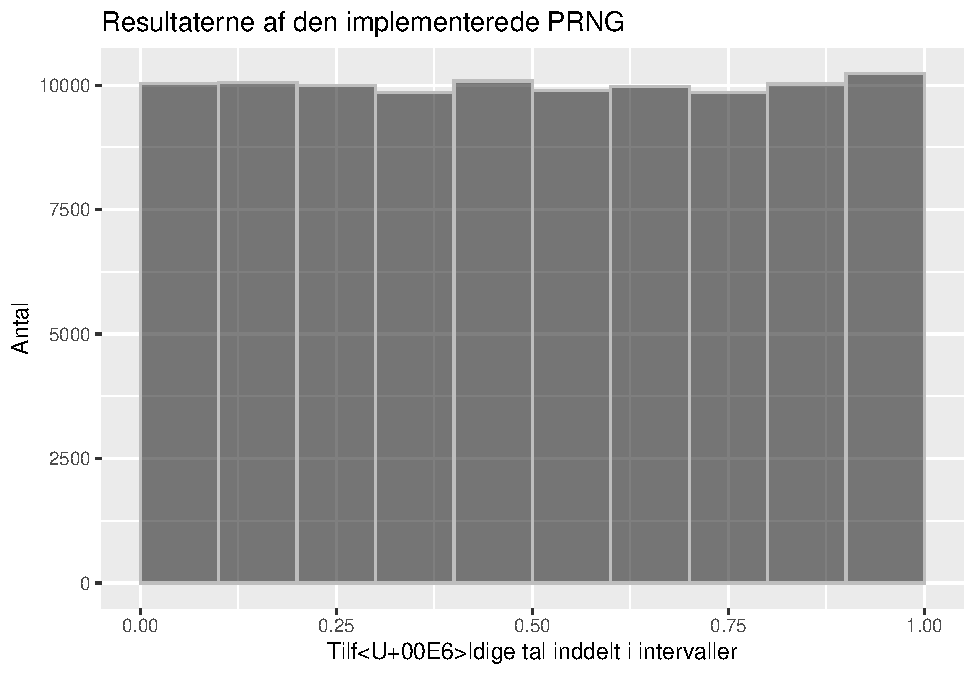
\includegraphics{TP2_files/figure-latex/Linear Congruence-1.pdf}

\#Uafhængige test

We use Pearson's Chi-squared Test of Independence to test if \(U{i}\) og
\(U{i + 1}\) in PRNG generated sequences are independent of each other.
Comparing observed frequencies is \(D=\sum_{i=1}^{k}(o_i-e_i)^2/e_i\) k
= the number of bins \(o_i\) = Observed frequency for ith bin \(e_i\) =
Expected frequency

When \(D\) score equals to zero, we will have an exact fit, D has a
chi-square distribution with k-1 degrees of freedom. Comparing \(D\)
score with \(\chi_[1-\alpha, k-1]\), if \(D\) is less we can pass with
confidence \(\alpha\)

\begin{Shaded}
\begin{Highlighting}[]
\NormalTok{obs }\OtherTok{\textless{}{-}} \FunctionTok{hist}\NormalTok{(}\FunctionTok{linear\_congruence}\NormalTok{(}\AttributeTok{i=}\DecValTok{10000}\NormalTok{, }\AttributeTok{X\_0 =} \DecValTok{1576}\NormalTok{))}\SpecialCharTok{$}\NormalTok{counts}
\end{Highlighting}
\end{Shaded}

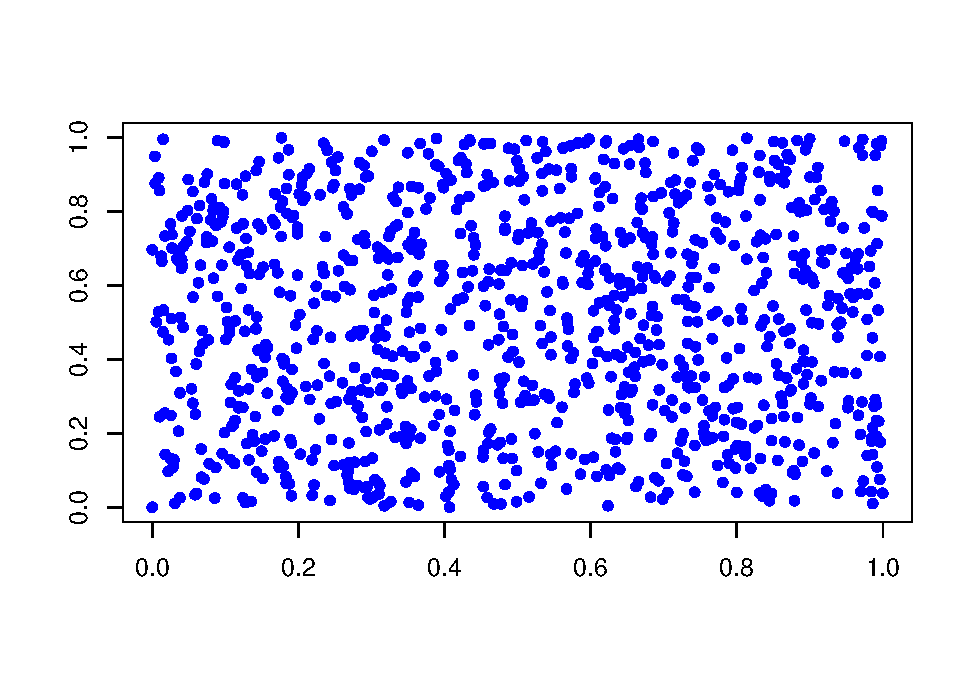
\includegraphics{TP2_files/figure-latex/unnamed-chunk-3-1.pdf}

\begin{Shaded}
\begin{Highlighting}[]
\NormalTok{exp }\OtherTok{\textless{}{-}}  \DecValTok{10000}\SpecialCharTok{/}\DecValTok{20}
\NormalTok{X\_squared }\OtherTok{\textless{}{-}} \FunctionTok{sum}\NormalTok{((obs}\SpecialCharTok{{-}}\NormalTok{exp)}\SpecialCharTok{\^{}}\DecValTok{2}\NormalTok{)}\SpecialCharTok{/}\NormalTok{exp}
\NormalTok{X\_significance }\OtherTok{\textless{}{-}} \FunctionTok{qchisq}\NormalTok{(}\FloatTok{0.95}\NormalTok{, }\DecValTok{19}\NormalTok{, }\AttributeTok{ncp =} \DecValTok{0}\NormalTok{, }\AttributeTok{lower.tail =} \ConstantTok{TRUE}\NormalTok{)}
\NormalTok{X\_squared }
\end{Highlighting}
\end{Shaded}

\begin{verbatim}
## [1] 15.74
\end{verbatim}

\begin{Shaded}
\begin{Highlighting}[]
\NormalTok{X\_significance}
\end{Highlighting}
\end{Shaded}

\begin{verbatim}
## [1] 30.14353
\end{verbatim}

It is observed that the observed difference is much smaller than
chi-squared value, therefore the LCG generated values follows a uniform
distribution with 95\% confidence.

\#Spektral test

Furthermore, the test result will be visualized by a spectral test. The
result shows a satisfactory level of randomness in the sequence
generated by PRNG.

\begin{Shaded}
\begin{Highlighting}[]
\NormalTok{spectral\_test }\OtherTok{\textless{}{-}} \ControlFlowTok{function}\NormalTok{()\{}
\NormalTok{  nSim }\OtherTok{=} \DecValTok{10000}
\NormalTok{  X }\OtherTok{=} \FunctionTok{rep}\NormalTok{(}\DecValTok{0}\NormalTok{,nSim)}
\NormalTok{  v1 }\OtherTok{\textless{}{-}} \FunctionTok{linear\_congruence}\NormalTok{(}\AttributeTok{i=}\DecValTok{10000}\NormalTok{, }\AttributeTok{X\_0 =} \DecValTok{1576}\NormalTok{)}
  \ControlFlowTok{for}\NormalTok{ (i }\ControlFlowTok{in} \DecValTok{2}\SpecialCharTok{:}\FunctionTok{length}\NormalTok{(v1))\{}
\NormalTok{   X[i] }\OtherTok{=}\NormalTok{ v1[i]}
\NormalTok{  \}}
\FunctionTok{plot}\NormalTok{(X[}\SpecialCharTok{{-}}\DecValTok{1}\NormalTok{]}\SpecialCharTok{/}\NormalTok{nSim,X[}\SpecialCharTok{{-}}\NormalTok{nSim]}\SpecialCharTok{/}\NormalTok{nSim,}\AttributeTok{col=}\StringTok{"blue"}\NormalTok{, }\AttributeTok{type=}\StringTok{"p"}\NormalTok{,}\AttributeTok{pch=}\DecValTok{20}\NormalTok{,}\AttributeTok{lwd=}\DecValTok{2}\NormalTok{)}
    
\NormalTok{\}}
\FunctionTok{spectral\_test}\NormalTok{()}
\end{Highlighting}
\end{Shaded}

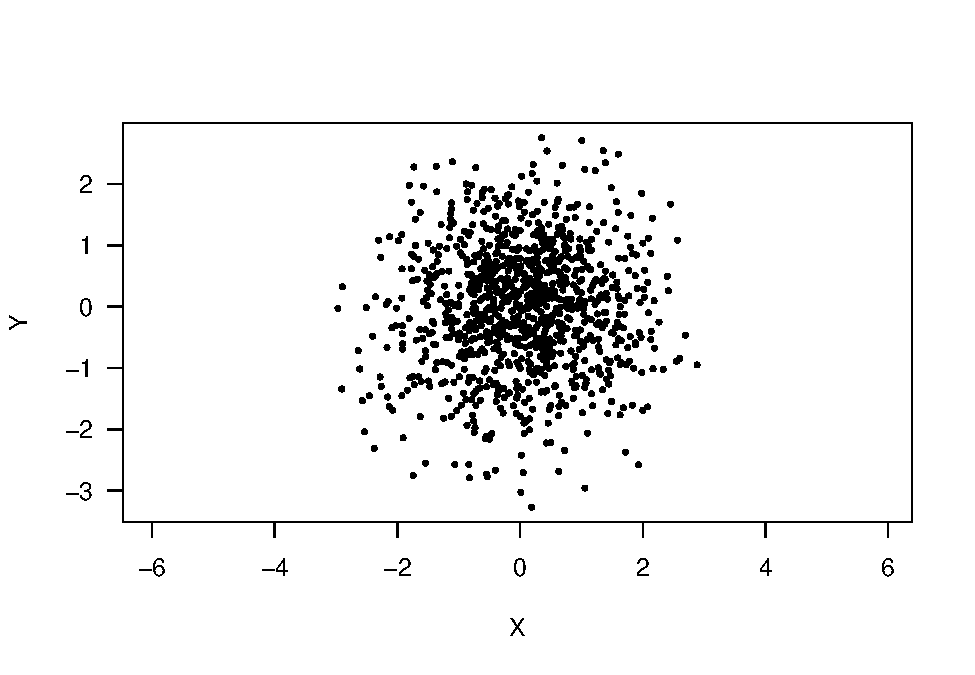
\includegraphics{TP2_files/figure-latex/unnamed-chunk-4-1.pdf}

\hypertarget{box-muller-transformation}{%
\section{Box-Muller transformation}\label{box-muller-transformation}}

Box-Muller transformationen er en metode, hvori to uniforme random
variabler transformeres til en normal fordeling. Den primære ide er at
ændre fra koordinatorne fra kartetiske til polære koordinator.

The principle idea is..instead of sampling independent Gaussians for the
x and y coordinates of the samples, we sample their independent uniform
angles and exponential squared distances to origin.

For two independent random variables x and y, the joint probability
density function \(f(x,y)\) is simply the product of density functions
f(x) and f(y).

Transformationen mellem kartetiske og polære-koordinator er:
\(x = cos(\theta)*r\) \(y = sin(\theta)*r\)

By writing the joint density function in polar cooridnates, 'the joint
PDF is the product of a constant \(1/2\pi\) and an exponential decay of
\(r^2\) with the parameter \(\lambda = 1/2\).

In pratices, \(U_1\) and \(U_2\) are uniform random variables, \(R^2\)
is calculated by applying the inverse CDF method to sample from an
exponential decay distribution with \(\lambda = 1/2\), which is
\(-2ln(U_1)\). \(\Theta\) is calculated from multiplying \(2\pi\) on
\(U_2\).

Dette svarer til at generere en tilfærdig vikel og en tilfældig radius,
som følger en ekponential fordeling, which means it is more likely to
generate distances closer to the origin, which is shown as

\begin{Shaded}
\begin{Highlighting}[]
\NormalTok{cartesian\_polar\_transform }\OtherTok{\textless{}{-}} \ControlFlowTok{function}\NormalTok{()\{}
\NormalTok{  uni\_rand\_num1 }\OtherTok{\textless{}{-}} \FunctionTok{linear\_congruence}\NormalTok{(}\AttributeTok{i=}\DecValTok{10000}\NormalTok{, }\AttributeTok{X\_0 =} \DecValTok{145}\NormalTok{)}
\NormalTok{  uni\_rand\_num2 }\OtherTok{\textless{}{-}} \FunctionTok{linear\_congruence}\NormalTok{(}\AttributeTok{i=}\DecValTok{10000}\NormalTok{, }\AttributeTok{X\_0 =} \DecValTok{7346}\NormalTok{)}
\NormalTok{  R }\OtherTok{\textless{}{-}} \FunctionTok{sqrt}\NormalTok{(}\SpecialCharTok{{-}}\DecValTok{2}\SpecialCharTok{*}\FunctionTok{log}\NormalTok{(uni\_rand\_num1))}
\NormalTok{  theta }\OtherTok{\textless{}{-}} \DecValTok{2}\SpecialCharTok{*}\NormalTok{pi}\SpecialCharTok{*}\NormalTok{uni\_rand\_num2}
\NormalTok{  X }\OtherTok{\textless{}{-}}\NormalTok{ R}\SpecialCharTok{*}\FunctionTok{cos}\NormalTok{(theta)}
\NormalTok{  Y }\OtherTok{\textless{}{-}}\NormalTok{ R}\SpecialCharTok{*}\FunctionTok{sin}\NormalTok{(theta)}
  \FunctionTok{plot}\NormalTok{(X,Y,}\AttributeTok{pch=}\DecValTok{19}\NormalTok{, }\AttributeTok{cex=}\FloatTok{0.4}\NormalTok{, }\AttributeTok{asp=}\DecValTok{1}\NormalTok{, }\AttributeTok{las=}\DecValTok{1}\NormalTok{)}
\NormalTok{\}}

\FunctionTok{cartesian\_polar\_transform}\NormalTok{()}
\end{Highlighting}
\end{Shaded}

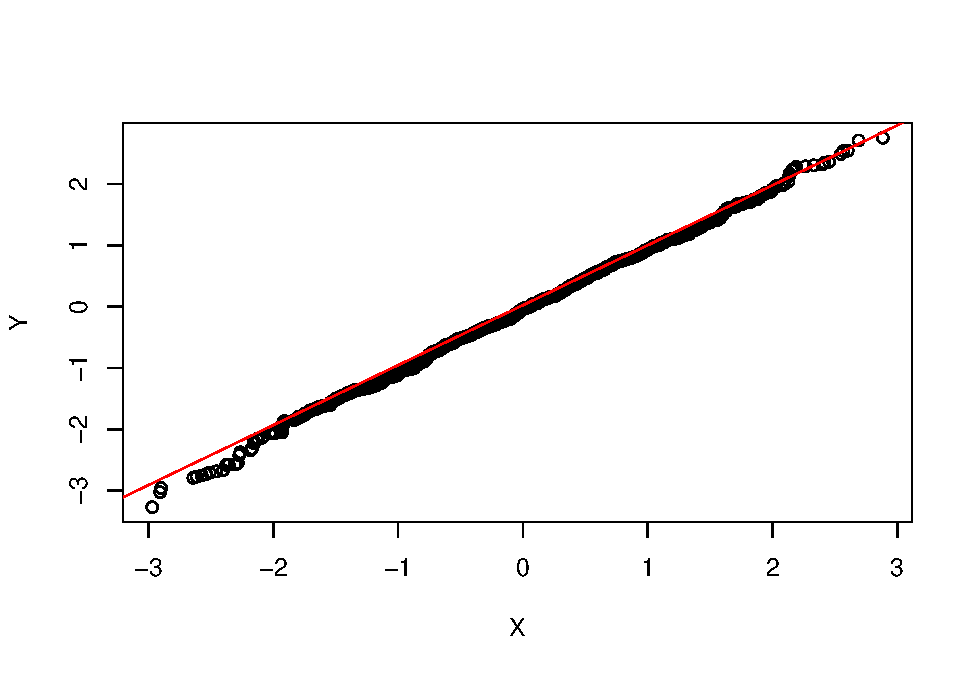
\includegraphics{TP2_files/figure-latex/unnamed-chunk-5-1.pdf}

\#Quantile-quantile plot

A Q--Q plot is a probability plot, which is a graphical method for
comparing two probability distributions by plotting their quantiles
against each other. we use qqplot to check the generated data X, Y
follows a normal distribution.

The result is most data points fall along a straight line, which means
data points of X,Y appears to be normally distributed.

\begin{Shaded}
\begin{Highlighting}[]
\NormalTok{qq\_normality\_check }\OtherTok{\textless{}{-}} \ControlFlowTok{function}\NormalTok{()\{}
\NormalTok{  uni\_rand\_num1 }\OtherTok{\textless{}{-}} \FunctionTok{linear\_congruence}\NormalTok{(}\AttributeTok{i=}\DecValTok{10000}\NormalTok{, }\AttributeTok{X\_0 =} \DecValTok{145}\NormalTok{)}
\NormalTok{  uni\_rand\_num2 }\OtherTok{\textless{}{-}} \FunctionTok{linear\_congruence}\NormalTok{(}\AttributeTok{i=}\DecValTok{10000}\NormalTok{, }\AttributeTok{X\_0 =} \DecValTok{7346}\NormalTok{)}
\NormalTok{  R }\OtherTok{\textless{}{-}} \FunctionTok{sqrt}\NormalTok{(}\SpecialCharTok{{-}}\DecValTok{2}\SpecialCharTok{*}\FunctionTok{log}\NormalTok{(uni\_rand\_num1))}
\NormalTok{  theta }\OtherTok{\textless{}{-}} \DecValTok{2}\SpecialCharTok{*}\NormalTok{pi}\SpecialCharTok{*}\NormalTok{uni\_rand\_num2}
\NormalTok{  X }\OtherTok{\textless{}{-}}\NormalTok{ R}\SpecialCharTok{*}\FunctionTok{cos}\NormalTok{(theta)}
\NormalTok{  Y }\OtherTok{\textless{}{-}}\NormalTok{ R}\SpecialCharTok{*}\FunctionTok{sin}\NormalTok{(theta)}
  \FunctionTok{qqplot}\NormalTok{(X, Y)}
\NormalTok{\}}

\FunctionTok{qq\_normality\_check}\NormalTok{()}
\end{Highlighting}
\end{Shaded}

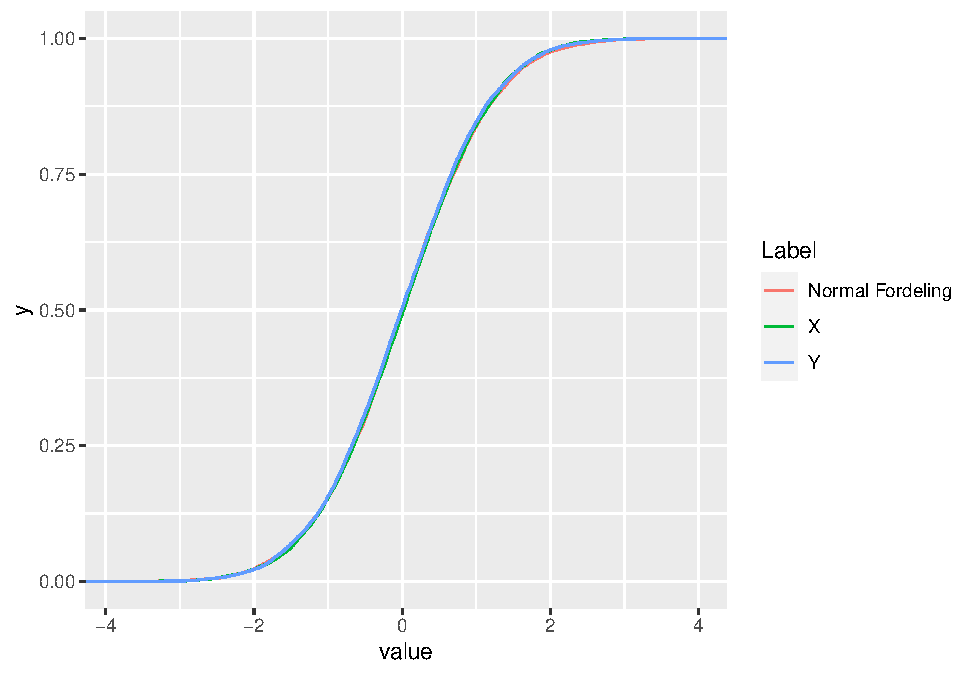
\includegraphics{TP2_files/figure-latex/unnamed-chunk-6-1.pdf}

\#Kolmogorov-Smirnov Test

Kolmogorov-Smirnov Test can be used to test sample of n observations is
from a continuous distribution. If the generated X, Y all follows a
normal distribution, the principle is that the difference between
observed CDF \(F_0(X)\) and expected CDF \(F_e(X)\) should be small.

The test statistics are \(K^+\), maximum observed deviation below the
expected cdf and \(K^-\), the minimum observed deviation below the
expected cdf.

\(K^+ = \sqrt(n)max(F_0(x) - F_e(x))\)

\(K^- = \sqrt(n)max(F_e(x) - F_0(x))\)

if \(K^+ < K[1-\alpha, n]\) and \(K^- < K[1-\alpha, n]\), test is passed
at \(\alpha\) level of significance.

Test Statistics \(D = Max|K^+, K^-|\)

\(F_e(x)\) is the theoretical freqency distribution, the normal
distribution cdf is \(F_X(x) = 1/2(1+erf(x-\mu/\sqrt2\sigma)\), while
the error funtion is defined as
\(erf(x) = 2/\sqrt\pi \int_{0}^{x}exp(-t^2)dt\)

We can firstly compare two cdfs visually

\begin{Shaded}
\begin{Highlighting}[]
\NormalTok{KS\_compare\_cdf }\OtherTok{\textless{}{-}} \ControlFlowTok{function}\NormalTok{()\{}
\NormalTok{  uni\_rand\_num1 }\OtherTok{\textless{}{-}} \FunctionTok{linear\_congruence}\NormalTok{(}\AttributeTok{i=}\DecValTok{10000}\NormalTok{, }\AttributeTok{X\_0 =} \DecValTok{145}\NormalTok{)}
\NormalTok{  uni\_rand\_num2 }\OtherTok{\textless{}{-}} \FunctionTok{linear\_congruence}\NormalTok{(}\AttributeTok{i=}\DecValTok{10000}\NormalTok{, }\AttributeTok{X\_0 =} \DecValTok{7346}\NormalTok{)}
\NormalTok{  R }\OtherTok{\textless{}{-}} \FunctionTok{sqrt}\NormalTok{(}\SpecialCharTok{{-}}\DecValTok{2}\SpecialCharTok{*}\FunctionTok{log}\NormalTok{(uni\_rand\_num1))}
\NormalTok{  theta }\OtherTok{\textless{}{-}} \DecValTok{2}\SpecialCharTok{*}\NormalTok{pi}\SpecialCharTok{*}\NormalTok{uni\_rand\_num2}
\NormalTok{  X }\OtherTok{\textless{}{-}}\NormalTok{ R}\SpecialCharTok{*}\FunctionTok{cos}\NormalTok{(theta)}
\NormalTok{  Y }\OtherTok{\textless{}{-}}\NormalTok{ R}\SpecialCharTok{*}\FunctionTok{sin}\NormalTok{(theta)}
\NormalTok{  n }\OtherTok{\textless{}{-}} \DecValTok{10}\SpecialCharTok{\^{}}\DecValTok{4}
\NormalTok{  samples }\OtherTok{\textless{}{-}} \FunctionTok{matrix}\NormalTok{(}\AttributeTok{ncol =} \DecValTok{2}\NormalTok{, }\AttributeTok{nrow =}\NormalTok{ n)}
\NormalTok{  samples[,}\DecValTok{1}\NormalTok{] }\OtherTok{\textless{}{-}}\NormalTok{ X}
\NormalTok{  samples[,}\DecValTok{2}\NormalTok{] }\OtherTok{\textless{}{-}}\NormalTok{ Y }
\NormalTok{  Label }\OtherTok{\textless{}{-}} \FunctionTok{rep}\NormalTok{(}\FunctionTok{c}\NormalTok{(}\StringTok{"x"}\NormalTok{, }\StringTok{"y"}\NormalTok{),n)}
\NormalTok{  value }\OtherTok{\textless{}{-}} \FunctionTok{c}\NormalTok{(samples[,}\DecValTok{1}\NormalTok{],samples[,}\DecValTok{2}\NormalTok{])}
\NormalTok{  df }\OtherTok{\textless{}{-}} \FunctionTok{data.frame}\NormalTok{(value, Label)}
  \FunctionTok{ggplot}\NormalTok{(df, }\FunctionTok{aes}\NormalTok{(}\AttributeTok{x=}\NormalTok{value)) }\SpecialCharTok{+} \FunctionTok{stat\_ecdf}\NormalTok{(}\FunctionTok{aes}\NormalTok{(}\AttributeTok{color=}\NormalTok{Label))}

\NormalTok{\}}

\FunctionTok{KS\_compare\_cdf}\NormalTok{()}
\end{Highlighting}
\end{Shaded}

\includegraphics{TP2_files/figure-latex/unnamed-chunk-7-1.pdf}

It can be observed that X,Y follows the cdf function for normal
distribution. However it could still be in our interest to run a
Kolmogorov-Smirnov test.

\begin{Shaded}
\begin{Highlighting}[]
\NormalTok{ks\_normality\_test }\OtherTok{\textless{}{-}} \ControlFlowTok{function}\NormalTok{()\{}
\NormalTok{  uni\_rand\_num1 }\OtherTok{\textless{}{-}} \FunctionTok{linear\_congruence}\NormalTok{(}\AttributeTok{i=}\DecValTok{10000}\NormalTok{, }\AttributeTok{X\_0 =} \DecValTok{145}\NormalTok{)}
\NormalTok{  uni\_rand\_num2 }\OtherTok{\textless{}{-}} \FunctionTok{linear\_congruence}\NormalTok{(}\AttributeTok{i=}\DecValTok{10000}\NormalTok{, }\AttributeTok{X\_0 =} \DecValTok{7346}\NormalTok{)}
\NormalTok{  R }\OtherTok{\textless{}{-}} \FunctionTok{sqrt}\NormalTok{(}\SpecialCharTok{{-}}\DecValTok{2}\SpecialCharTok{*}\FunctionTok{log}\NormalTok{(uni\_rand\_num1))}
\NormalTok{  theta }\OtherTok{\textless{}{-}} \DecValTok{2}\SpecialCharTok{*}\NormalTok{pi}\SpecialCharTok{*}\NormalTok{uni\_rand\_num2}
\NormalTok{  X }\OtherTok{\textless{}{-}}\NormalTok{ R}\SpecialCharTok{*}\FunctionTok{cos}\NormalTok{(theta)}
\NormalTok{  Y }\OtherTok{\textless{}{-}}\NormalTok{ R}\SpecialCharTok{*}\FunctionTok{sin}\NormalTok{(theta)}
  \FunctionTok{ks.test}\NormalTok{(X,}\StringTok{\textquotesingle{}pnorm\textquotesingle{}}\NormalTok{)}
  \FunctionTok{ks.test}\NormalTok{(Y, }\StringTok{\textquotesingle{}pnorm\textquotesingle{}}\NormalTok{) }\CommentTok{\#value for X is already returned}
\NormalTok{\}}

\FunctionTok{ks\_normality\_test}\NormalTok{()}
\end{Highlighting}
\end{Shaded}

\begin{verbatim}
## 
##  One-sample Kolmogorov-Smirnov test
## 
## data:  Y
## D = 0.011159, p-value = 0.1657
## alternative hypothesis: two-sided
\end{verbatim}

We firstly run KS test to examine if X is from a normal distribution,
then run KS test to check if the two distributions are critical values
for KS test is 0.04301, D score is smaller than the critical score,
therefore we confirm that data are normally distributed.

Ud af dette, fås der to tal \(x\) og \(y\), som i dette tilfælde er
uafhængige tilfældige variabler med en normalfordeling. Resultater X,Y
er to uafhægige normal fordelinger. Forneden kan resultaterne af
Box-Muller transformationen ses:

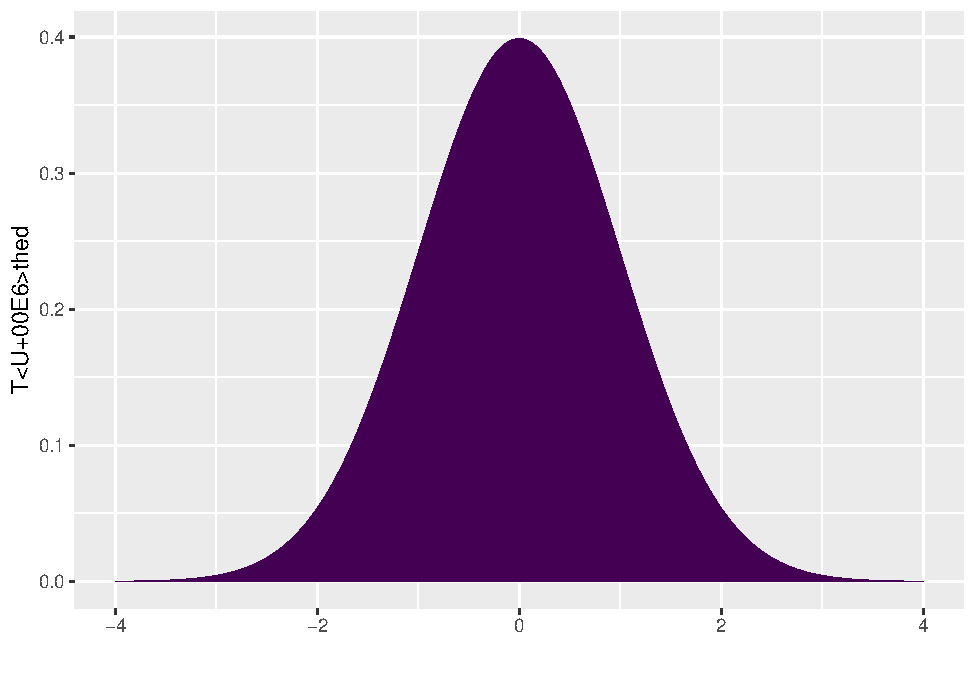
\includegraphics{TP2_files/figure-latex/unnamed-chunk-9-1.pdf}

\hypertarget{teori}{%
\section{Teori}\label{teori}}

\hypertarget{middelvuxe6rdi-og-standardafvigelse}{%
\subsection{Middelværdi og
standardafvigelse}\label{middelvuxe6rdi-og-standardafvigelse}}

I en population findes der to værdier, \(\mu\) og \(\sigma\), som er
interessante at kigge nærmere på. Gennemsnittet af en population kaldes
\(\mu\), mens at populationens standardafvigelse kaldes \(\sigma\).

Populations standardafvigelse kan udregnes ud fra populationens varians.
Nedenstående ligning viser hvordan variansen for en stikprøve kan
udregnes:

\[
\begin{aligned}
var(x)=s^2 = \sum_{i=1}^{n} \frac{(x_i-\overline{x})^2}{n}
\end{aligned}
\] Herunder er der: - \(x_i\), som svarer til den enkelte observation i
stikprøven. - \(\overline{x}\), som svarer til gennemsnittet af
stikprøven.

Sammenhænget mellem en populations standardafvigelse og populationens
varians kan ses i nedenstående ligning.: \[
\begin{aligned}
\sigma=\sqrt{var(X)}=\sqrt{\sigma^2}
\end{aligned}
\] Populationen bliver her betegnet som X.

\hypertarget{fordelinger}{%
\subsection{Fordelinger}\label{fordelinger}}

Der findes en lang række sandynlighedsfordelinger og i det følgende
afsnit fokuseres der på de fordelinger, som har mest relevans for
projektet.

\hypertarget{standardnormalfordeling}{%
\subsubsection{Standardnormalfordeling}\label{standardnormalfordeling}}

\begin{itemize}
\tightlist
\item
  Billede: En standardnormalfordeling er kendetegnet ved at \(\mu=0\),
  og at \(\sigma = 1\). Desuden har en standardnormalfordeling et
  klokkeformet udseende. Nedenstående er der plottet en
  standardnormalfordeling:
\end{itemize}

\begin{Shaded}
\begin{Highlighting}[]
\FunctionTok{qdist}\NormalTok{(}\StringTok{"norm"}\NormalTok{,}\AttributeTok{p=}\DecValTok{1}\NormalTok{,}\AttributeTok{mean =} \DecValTok{0}\NormalTok{, }\AttributeTok{sd =} \DecValTok{1}\NormalTok{,}\AttributeTok{xlim =} \FunctionTok{c}\NormalTok{(}\SpecialCharTok{{-}}\DecValTok{4}\NormalTok{,}\DecValTok{4}\NormalTok{))}
\end{Highlighting}
\end{Shaded}

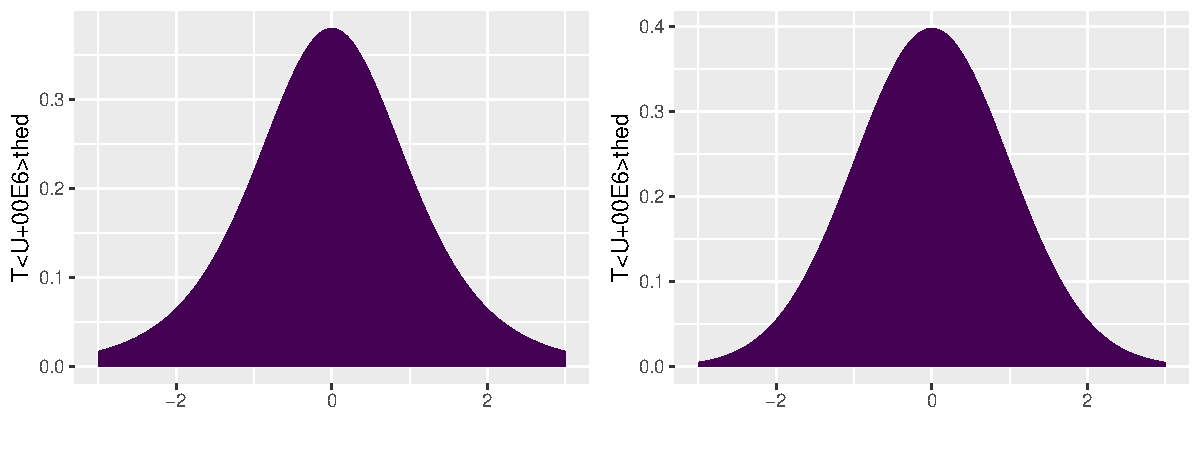
\includegraphics{TP2_files/figure-latex/unnamed-chunk-10-1.pdf}

\begin{verbatim}
## [1] Inf
\end{verbatim}

Der er en høj sandsynlighed for at få et værdi tæt på 0. Jo længere man
afviger fra \(\mu\), jo mindre er densiteten,som medfører at
sandsynligheden for de givne værdier mindskes. Ergo vil sandsynligheden
for at få 2, være mindre end sansynligheden for at få 0. En af
anveldeserne for en standarnormalfordeling er at den kan benyttes til en
Z-test, som benyttes senere i projektet.

\hypertarget{z-fordeling}{%
\paragraph{Z-fordeling}\label{z-fordeling}}

For at finde z-scoren, skal \(\mu,\sigma\) være kendt. Z-scoren kan
udregnes for normalfordelinger ved formlen: \[
\begin{aligned}
z = \frac{y-\mu}\sigma
\end{aligned}
\] hvor \(y\) er en værdi, som er \(z\) standardafvigelser fra \(\mu\)
Desuden, kan det udledes, at hvis \(z>0\) er y-værdien på højre side af
\(\mu\), og omvendt, hvis \(z<0\), er y-værdien på venstre side af
\(\mu\).

\hypertarget{t-fordeling}{%
\paragraph{T-fordeling}\label{t-fordeling}}

En T-fordeling laves ud fra en standardnormalfordeling og dens udseende
minder også om denne fordeling. Forskellen på en T-fordeling og en
standardnormalfordeling, ligger i, at en T-fordeling laves ud fra
frihedsgrader. For en stikprøve vil antallet af frihedsgrader være
antallet af observationer minus 1, altså \(n-1\). Jo flere frihedsgrader
der er, jo mere ligner en T-fordeling en standardnormalfordeling.
Nedenstående er der plottet 2 T-fordelinger med henholdsvis 5 og 100
frihedsgrader:

\begin{Shaded}
\begin{Highlighting}[]
\NormalTok{p1 }\OtherTok{\textless{}{-}} \FunctionTok{qdist}\NormalTok{(}\StringTok{"t"}\NormalTok{, }\AttributeTok{df =} \DecValTok{5}\NormalTok{, }\AttributeTok{p =} \DecValTok{1}\NormalTok{, }\AttributeTok{return =} \StringTok{"plot"}\NormalTok{)}
\NormalTok{p2 }\OtherTok{\textless{}{-}} \FunctionTok{qdist}\NormalTok{(}\StringTok{"t"}\NormalTok{, }\AttributeTok{df =} \DecValTok{100}\NormalTok{, }\AttributeTok{p =} \DecValTok{1}\NormalTok{, }\AttributeTok{return =} \StringTok{"plot"}\NormalTok{)}
\CommentTok{\#p3 \textless{}{-} qdist(mean = 0, sd = 1, p = 0, return="plot")}
\FunctionTok{grid.arrange}\NormalTok{(p1, p2, }\AttributeTok{ncol=}\DecValTok{2}\NormalTok{)}
\end{Highlighting}
\end{Shaded}

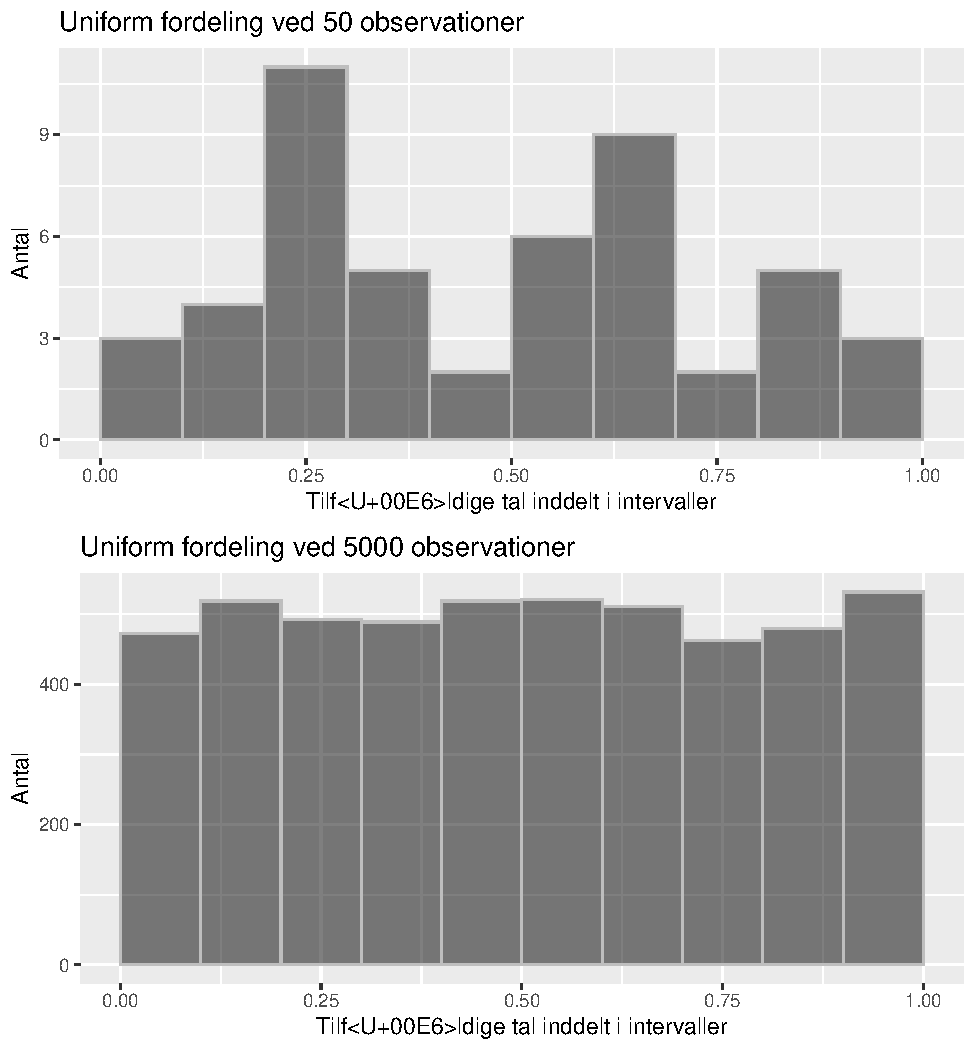
\includegraphics{TP2_files/figure-latex/unnamed-chunk-11-1.pdf}

\hypertarget{binomialfordeling}{%
\subsubsection{Binomialfordeling}\label{binomialfordeling}}

Binomialfordelingen benyttes i sammenhænge med kvalitative data.
Specifikt er der kun to mulige udfald. Hvis der er lige stor chance for
hvert af udfaldene, altså \(\pi = 0.50\), og en stor stikprøve, vil en
binomialfordeling vise sig at være symmetrisk. Nedenstående er et
eksempel på 4 binomialfordelinger.

\begin{Shaded}
\begin{Highlighting}[]
\FunctionTok{set.seed}\NormalTok{(}\DecValTok{987}\NormalTok{)}
\NormalTok{rbino1 }\OtherTok{\textless{}{-}} \FunctionTok{c}\NormalTok{(}\FunctionTok{rbinom}\NormalTok{(}\DecValTok{100}\NormalTok{, }\DecValTok{20}\NormalTok{, }\FloatTok{0.5}\NormalTok{))}
\NormalTok{p1 }\OtherTok{\textless{}{-}} \FunctionTok{gf\_histogram}\NormalTok{(}\SpecialCharTok{\textasciitilde{}}\NormalTok{ rbino1, }\AttributeTok{fill=}\StringTok{"black"}\NormalTok{, }\AttributeTok{col=}\StringTok{"grey"}\NormalTok{, }\AttributeTok{breaks =} \FunctionTok{seq}\NormalTok{(}\DecValTok{2}\NormalTok{,}\DecValTok{18}\NormalTok{, }\AttributeTok{by=}\DecValTok{1}\NormalTok{), }\AttributeTok{title =} \StringTok{"Kontrol"}\NormalTok{, }\AttributeTok{xlab =} \StringTok{""}\NormalTok{) }\CommentTok{\#Test 1: Grundtest,(20 mønter kastes 100 gange)}


\CommentTok{\#Test 2: Antallet af test forøges}
\FunctionTok{set.seed}\NormalTok{(}\DecValTok{987}\NormalTok{)}
\NormalTok{rbino2 }\OtherTok{\textless{}{-}} \FunctionTok{c}\NormalTok{(}\FunctionTok{rbinom}\NormalTok{(}\DecValTok{10000}\NormalTok{,}\DecValTok{20}\NormalTok{,}\FloatTok{0.5}\NormalTok{))}
\NormalTok{p2 }\OtherTok{\textless{}{-}} \FunctionTok{gf\_histogram}\NormalTok{(}\SpecialCharTok{\textasciitilde{}}\NormalTok{ rbino2, }\AttributeTok{fill =} \StringTok{"black"}\NormalTok{, }\AttributeTok{col =} \StringTok{"grey"}\NormalTok{, }\AttributeTok{breaks =} \FunctionTok{seq}\NormalTok{(}\DecValTok{2}\NormalTok{,}\DecValTok{18}\NormalTok{, }\AttributeTok{by =}\DecValTok{1}\NormalTok{), }\AttributeTok{title =} \StringTok{"T1"}\NormalTok{, }\AttributeTok{xlab =} \StringTok{""}\NormalTok{) }

\CommentTok{\#Test 3: Antallet af kroner forøges}
\FunctionTok{set.seed}\NormalTok{(}\DecValTok{987}\NormalTok{)}
\NormalTok{rbino3 }\OtherTok{\textless{}{-}} \FunctionTok{c}\NormalTok{(}\FunctionTok{rbinom}\NormalTok{(}\DecValTok{100}\NormalTok{,}\DecValTok{30}\NormalTok{,}\FloatTok{0.5}\NormalTok{))}
\NormalTok{p3 }\OtherTok{\textless{}{-}} \FunctionTok{gf\_histogram}\NormalTok{(}\SpecialCharTok{\textasciitilde{}}\NormalTok{ rbino3, }\AttributeTok{fill =} \StringTok{"black"}\NormalTok{, }\AttributeTok{col =} \StringTok{"grey"}\NormalTok{, }\AttributeTok{breaks =} \FunctionTok{seq}\NormalTok{(}\DecValTok{5}\NormalTok{,}\DecValTok{25}\NormalTok{, }\AttributeTok{by =}\DecValTok{1}\NormalTok{), }\AttributeTok{title =} \StringTok{"T2"}\NormalTok{, }\AttributeTok{xlab =} \StringTok{""}\NormalTok{) }

\CommentTok{\#Test 4: Sandsynligheden ændres fra 50\%}
\FunctionTok{set.seed}\NormalTok{(}\DecValTok{987}\NormalTok{)}
\NormalTok{rbino4 }\OtherTok{\textless{}{-}} \FunctionTok{c}\NormalTok{(}\FunctionTok{rbinom}\NormalTok{(}\DecValTok{100}\NormalTok{,}\DecValTok{20}\NormalTok{,}\FloatTok{0.3}\NormalTok{))}
\NormalTok{p4 }\OtherTok{\textless{}{-}} \FunctionTok{gf\_histogram}\NormalTok{(}\SpecialCharTok{\textasciitilde{}}\NormalTok{ rbino4, }\AttributeTok{fill =} \StringTok{"black"}\NormalTok{, }\AttributeTok{col =} \StringTok{"grey"}\NormalTok{, }\AttributeTok{breaks =} \FunctionTok{seq}\NormalTok{(}\DecValTok{0}\NormalTok{,}\DecValTok{11}\NormalTok{, }\AttributeTok{by =}\DecValTok{1}\NormalTok{), }\AttributeTok{title =} \StringTok{"T3"}\NormalTok{, }\AttributeTok{xlab =} \StringTok{""}\NormalTok{) }

\FunctionTok{grid.arrange}\NormalTok{(p1, p2, p3, p4,}\AttributeTok{ncol=}\DecValTok{2}\NormalTok{,}\AttributeTok{nrow =} \DecValTok{2}\NormalTok{)}
\end{Highlighting}
\end{Shaded}

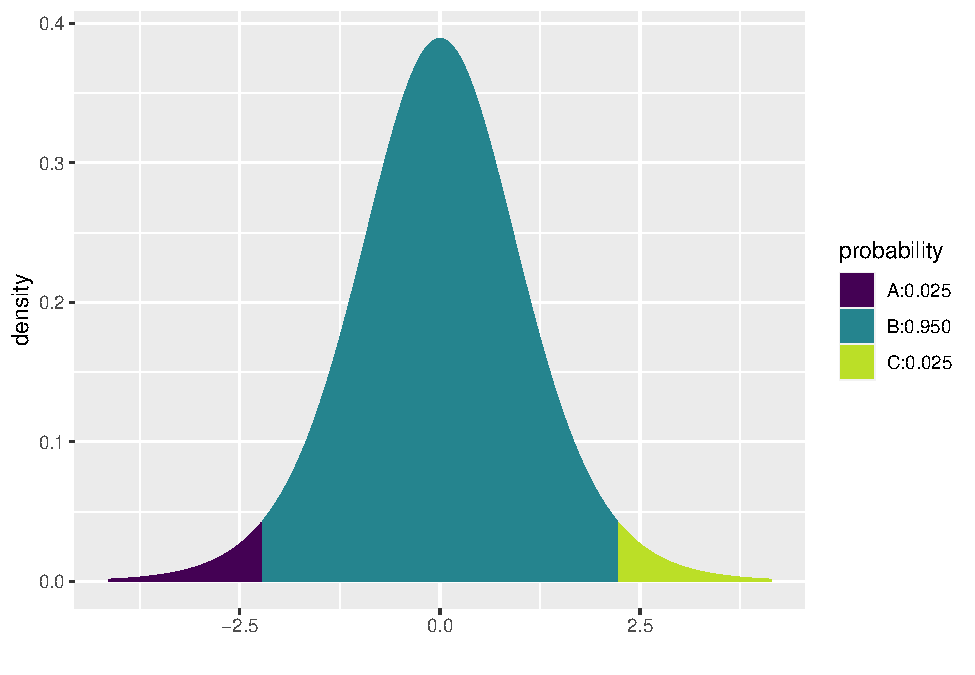
\includegraphics{TP2_files/figure-latex/unnamed-chunk-12-1.pdf} I
ovenstående figur er der altså fire grafer, som er lavet ud fra
binomialfordelingen. Der er en kontrolgraf, hvor 100 observationer hver
bliver testet 20 gange med en \(50\%\) chance for success. Yderligere er
der T1, T2 og T3, hvor der ved hver graf er ændret en af parameterene
fra kontrol grafen. T1 har flere observationer, som gør at grafen får et
udseende af en normalfordeling, her kan det aflæses at
\(\overline{x} = 10\). Ved T2 bliver hver observation testet 30 gange i
stedet for 20 gange, og dette resulterer i at middelværdien (hvis
antallet af observationer er stort nok) i stedet vil være
\(\overline{x} = 15\). I T3 er sandsynligheden for success ændret fra
\(50\%\) til \(30\%\). Dette ændrer igen udseendet på grafen, hvor
middelværdien bliver lavere, da hver test har en mindre sandsynlighed
for at være en success. \[
\begin{aligned}
\hat\pi = \frac{x}n
\end{aligned}
\]

\hypertarget{poisson-fordeling}{%
\subsubsection{Poisson Fordeling}\label{poisson-fordeling}}

En poisson fordeling beskriver chancen for at en begivenhed sker et
givet antal gange over et kendt tidsinterval. Dette kunne være hvor
mange gange der har været stormvejr indenfor det sidste år. Fordelingen
laves ud fra følgende formel: \[
\begin{aligned}
P(x;\lambda) = \frac{(e^{-\lambda}\cdot\lambda^x)}{x!}
\end{aligned}
\] Hvor: - \(e\) er eulers tal. - \(\lambda\) er begivenhedsraten, altså
det forventede antal gange begivenheden vil ske.

Hvis \(lambda\) er 5, og der ndersøges hvad chancen for at begivenheden
sker 7 gange, så vil \(x=7\). Dette eksempel kan ses forneden:

\begin{Shaded}
\begin{Highlighting}[]
\NormalTok{(}\FunctionTok{exp}\NormalTok{(}\DecValTok{1}\NormalTok{)}\SpecialCharTok{\^{}{-}}\DecValTok{5}\SpecialCharTok{*}\DecValTok{5}\SpecialCharTok{\^{}}\DecValTok{7}\NormalTok{)}\SpecialCharTok{/}\FunctionTok{factorial}\NormalTok{(}\DecValTok{7}\NormalTok{)}
\end{Highlighting}
\end{Shaded}

\begin{verbatim}
## [1] 0.1044449
\end{verbatim}

Der er altså en \(10.4\%\) chance for at en begivenhed sker 7 gange,
hvis begivenhedsraten er 5. Nedenstående er resultaterne af denne
poissonfordeling plottet:

\begin{Shaded}
\begin{Highlighting}[]
\NormalTok{sucess }\OtherTok{\textless{}{-}} \DecValTok{0}\SpecialCharTok{:}\DecValTok{20}
\FunctionTok{dpois}\NormalTok{(}\DecValTok{7}\NormalTok{, }\DecValTok{5}\NormalTok{)}
\end{Highlighting}
\end{Shaded}

\begin{verbatim}
## [1] 0.1044449
\end{verbatim}

\begin{Shaded}
\begin{Highlighting}[]
\FunctionTok{plot}\NormalTok{(sucess, }\FunctionTok{dpois}\NormalTok{(}\DecValTok{0}\SpecialCharTok{:}\DecValTok{20}\NormalTok{, }\DecValTok{5}\NormalTok{), }\AttributeTok{type =} \StringTok{"h"}\NormalTok{, }\AttributeTok{xlab =} \StringTok{""}\NormalTok{, }\AttributeTok{ylab =} \StringTok{""}\NormalTok{)}
\end{Highlighting}
\end{Shaded}

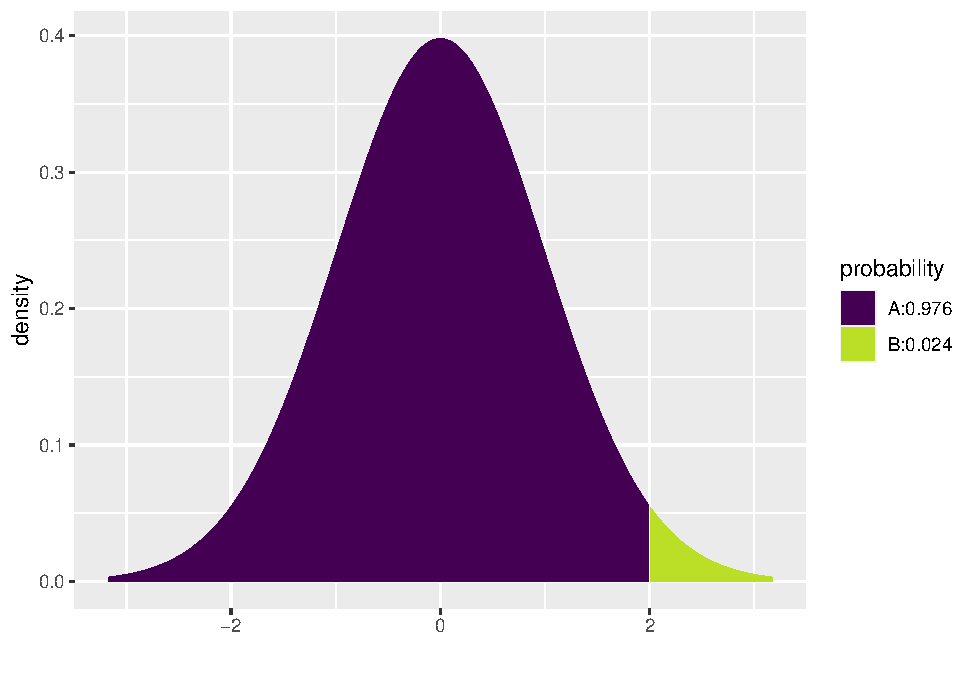
\includegraphics{TP2_files/figure-latex/unnamed-chunk-14-1.pdf}

\hypertarget{uniform-fordeling}{%
\subsubsection{Uniform fordeling}\label{uniform-fordeling}}

En uniform fordeling, er hvor dataet bliver indelt i lige store
intervaller, og alle intervaller, har lige antal observationer. Det er
vigtigt at notere at hvis antallet af observationer er lavt, vil
fordelingen ikke tilsyneladende være uniform. Dette vises ved at lave to
uniformfordelinger på det samme seed,hvor den eneste forskel er antallet
af observationer. Dette kan ses i de nedenstående grafer.

\begin{Shaded}
\begin{Highlighting}[]
\FunctionTok{set.seed}\NormalTok{(}\DecValTok{1234}\NormalTok{)}
\NormalTok{unifx }\OtherTok{\textless{}{-}} \FunctionTok{runif}\NormalTok{(}\DecValTok{50}\NormalTok{,}\AttributeTok{min =} \DecValTok{0}\NormalTok{, }\AttributeTok{max =}\DecValTok{1}\NormalTok{)}
\FunctionTok{set.seed}\NormalTok{(}\DecValTok{1234}\NormalTok{)}
\NormalTok{unifx1 }\OtherTok{\textless{}{-}} \FunctionTok{runif}\NormalTok{(}\DecValTok{5000}\NormalTok{, }\AttributeTok{min =} \DecValTok{0}\NormalTok{, }\AttributeTok{max =} \DecValTok{1}\NormalTok{)}

\NormalTok{p1 }\OtherTok{\textless{}{-}} \FunctionTok{gf\_histogram}\NormalTok{(}\SpecialCharTok{\textasciitilde{}}\NormalTok{unifx,}\AttributeTok{breaks =} \FunctionTok{seq}\NormalTok{(}\DecValTok{0}\NormalTok{,}\DecValTok{1}\NormalTok{,}\AttributeTok{by=}\FloatTok{0.1}\NormalTok{), }\AttributeTok{fill=}\StringTok{"black"}\NormalTok{, }\AttributeTok{col=}\StringTok{"grey"}\NormalTok{,}\AttributeTok{xlab =} \StringTok{"tilfældige tal inddelt i intervaller"}\NormalTok{, }\AttributeTok{ylab =} \StringTok{"antal"}\NormalTok{, }\AttributeTok{title =} \StringTok{"Uniform fordeling ved 50 observationer"}\NormalTok{)}
\NormalTok{p2 }\OtherTok{\textless{}{-}} \FunctionTok{gf\_histogram}\NormalTok{(}\SpecialCharTok{\textasciitilde{}}\NormalTok{unifx1,}\AttributeTok{breaks =} \FunctionTok{seq}\NormalTok{(}\DecValTok{0}\NormalTok{,}\DecValTok{1}\NormalTok{,}\AttributeTok{by=}\FloatTok{0.1}\NormalTok{), }\AttributeTok{fill=}\StringTok{"black"}\NormalTok{, }\AttributeTok{col=}\StringTok{"grey"}\NormalTok{,}\AttributeTok{xlab =} \StringTok{"tilfældige tal inddelt i intervaller"}\NormalTok{, }\AttributeTok{ylab =} \StringTok{"antal"}\NormalTok{, }\AttributeTok{title =} \StringTok{"Uniform fordeling ved 5000 observationer"}\NormalTok{)}
\FunctionTok{grid.arrange}\NormalTok{(p1, p2, }\AttributeTok{nrow=}\DecValTok{2}\NormalTok{)}
\end{Highlighting}
\end{Shaded}

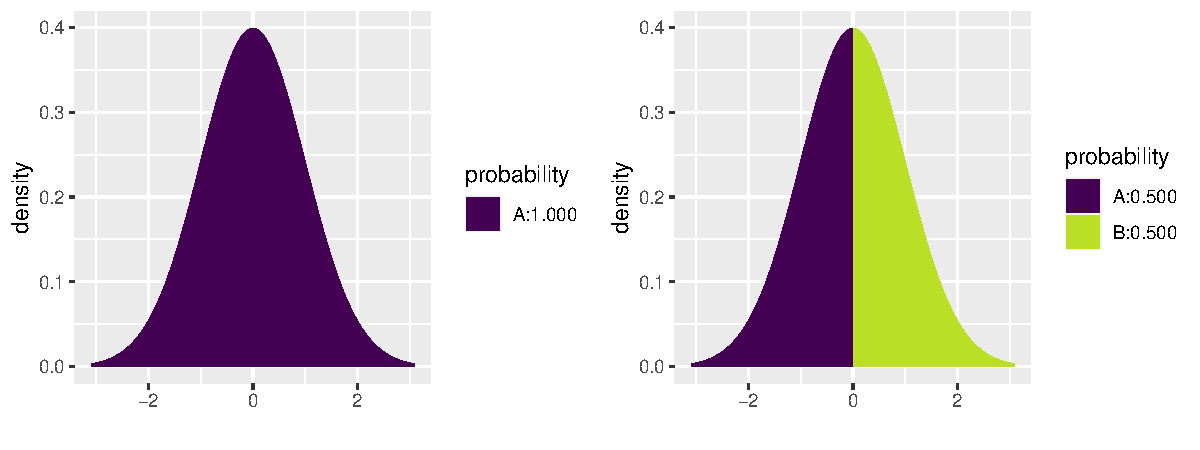
\includegraphics{TP2_files/figure-latex/unnamed-chunk-15-1.pdf}

\hypertarget{clt}{%
\subsection{CLT}\label{clt}}

\hypertarget{statistisk-inferens}{%
\subsection{Statistisk inferens}\label{statistisk-inferens}}

Indenfor statistisk analyse er der to kategorier; den første, deskriptiv
statistik har i fokus at beskrive data, hvor den anden statistisk
inferens har i fokus at lave forudsigelser om et element på baggrund af
data og tendenser dertil. I rapporten anvendes statistisk inferens, det
gøres i form af estimation, der benyttes både punktestimater og
intervalestimater, hvilket vil sige, at der først findes et
punktestimat, altså et gæt, eksemplificeret ved middelværdien fra en
stikprøve. Selvom der så er meget meget lille sandsynlighed for, at det
også er middelværdien i hele populationen, kan estimatet anvendes, til
at lave et intervalestimat, eller et konfidensinterval, hvori hele
populationens middelværdi med ret stor sikkerhed hører til.

\hypertarget{konfidensinterval}{%
\subsubsection{Konfidensinterval}\label{konfidensinterval}}

Når der indenfor statistik estimeres på en populations parameter ud fra
en stikprøve, vil resultatet aldrig være perfekt. Dette skyldes at der
er en fejlmargin, som der skal tages højde fra. En måde hvorpå man kan
tage højde for denne fejlmargin er et konfidensinterval.

Et konfidensinterval for en givet parameter er et interval mellem to
tal, hvori det estimeres at parameteren ligger i. Sandsynligheden for at
producere et interval som indeholder parameteren kaldes for et
konfidensniveau. Denne værdi er valgt til et tal tæt på 1, som regel
enten 0.95 eller 0.99.

En konfidensinterval skabes på baggrund af et punktestimat og
fejlmarginen. Måden dette gøres på, kan ses forneden: \[
\begin{aligned}
KI = Punktestimat \; \pm \; fejlmargin
\end{aligned}
\] Måden at finde konfidensintervallet varierer baseret på hvilket
fordeling man bruger. I de følgende afsnit vil der forklares hvordan
konfidensintervallet for kvalitative og kvantitative variabler findes og
opstilles ved hjælp af eksempler.

\hypertarget{kvalitative-variabler}{%
\paragraph{Kvalitative variabler}\label{kvalitative-variabler}}

Hvis man spurgte en population hvorvidt de kunne lide deres job eller
ej, ville en andel svare ``ja'' og en andel svare ``nej''. Er man
interesseret i hvor mange procent svarede ``ja'' til spørgsmålet, ville
man dividere antallet der svarede ``ja'' med antallet af observation. Se
følgende: \[
\begin{aligned}
\hat{\pi}_{ja} = \frac{n_{ja}}{n{_{total}}}
\end{aligned}
\] Før selve konfidensintervallet kan opstilles, skal standardfejlen
(\(sf\)) findes. Følgende formel bruges for at finde standardfejlen for
kvalitative variabler: \[
\begin{aligned}
sf(\hat{\pi}) = \sqrt{\frac{\hat{\pi}(1-\hat{\pi})}n{}}
\end{aligned}
\] Når standardfejlen er fundet, kan denne ganges med en værdi som
afhænger af signifikansniveauet. Denne værdi kaldes \(z_{crit}\). For at
finde ud af hvilken værdi \(z_{crit}\) skal være, benyttes en z-test. En
z-test er i realiteten bare en standardnormalfordeling. For at finde
\(z_{crit}\) for signifikansniveauet 95\%, findes x-værdien ved 97.5\%
og 2.5\%.

\begin{Shaded}
\begin{Highlighting}[]
\FunctionTok{qdist}\NormalTok{(}\StringTok{"norm"}\NormalTok{, }\AttributeTok{mean =} \DecValTok{0}\NormalTok{, }\AttributeTok{sd =} \DecValTok{1}\NormalTok{, }\AttributeTok{p =} \FunctionTok{c}\NormalTok{(}\FloatTok{0.025}\NormalTok{,}\FloatTok{0.975}\NormalTok{))}
\end{Highlighting}
\end{Shaded}

\includegraphics{TP2_files/figure-latex/unnamed-chunk-16-1.pdf}

\begin{verbatim}
## [1] -1.959964  1.959964
\end{verbatim}

Denne værdi aflæses til at være \textasciitilde1.96. Nu kan
konfidensintervallet opstilles via følgende ligning: \[
\begin{aligned}
KI = \hat{\pi}\; \pm 1.96\cdot sf(\hat{\pi})
\end{aligned}
\] Da dette blev lavet udfra signifikansniveauet 95\%, kan der altså med
95\%'s sikkerhed siges at \(\hat\pi\) ligger indenfor intervallet: \[
\begin{aligned}
(\hat\pi\;-1.96\;\cdot sf(\hat\pi) \ \ ,\ \  \hat\pi \; + 1.96\;\cdot sf(\hat\pi))
\end{aligned}
\]

\hypertarget{kvantitative-variabler}{%
\paragraph{Kvantitative variabler}\label{kvantitative-variabler}}

Konfidensintervallet for kvantitative variabler har næsten samme formel
som ved kvalitative variabler. Dog er måden hvorpå standardfejlen findes
anderledes. Desuden skal der bruges en anden slags test ved hjælp af
signifikansniveauet.

\[
\begin{aligned}
KI = \overline{y}\;\pm t_{crit} \;\cdot sf(\overline{y})
\end{aligned}
\] Herunder er standardfejlen udregnet ved: \[
\begin{aligned}
sf(\overline{y}) = \frac{s}{\sqrt{n}}
\end{aligned}
\] hvor s er standardafvigelsen for stikprøven og n er antallet af
observationer i stikprøven.

For at finde \(t_{crit}\) benyttes der en t-test. Hvis det ønskede
signifikansniveau igen er 95\% hvor der igen aflæses x-værdien ved
\(2.5\%\) og \(97.5\%\). Nedenstående er der et eksempel, hvor en t-test
med 50 frihedsgrader benyttes til at finde 95\% signifikansniveauet:

\begin{Shaded}
\begin{Highlighting}[]
\FunctionTok{qdist}\NormalTok{(}\StringTok{"t"}\NormalTok{, }\AttributeTok{df =} \DecValTok{50}\NormalTok{, }\AttributeTok{p =} \FunctionTok{c}\NormalTok{(}\FloatTok{0.025}\NormalTok{,}\FloatTok{0.975}\NormalTok{))}
\end{Highlighting}
\end{Shaded}

\includegraphics{TP2_files/figure-latex/unnamed-chunk-17-1.pdf}

\begin{verbatim}
## [1] -2.008559  2.008559
\end{verbatim}

Denne værdi aflæses til at være \textasciitilde2.01. Nu kan
konfidensintervallet igen opstilles: \[
\begin{aligned}
(\overline{x}\;-2.01 \;\cdot sf(\overline{x}) \ \ , \ \ \overline{x}\;+2.01 \;\cdot sf(\overline{x})
\end{aligned}
\]

\hypertarget{hypoteser}{%
\subsubsection{Hypoteser}\label{hypoteser}}

Hver signifikanstest har to hypoteser. En hypotese er et udsagn omkring
værdien af population parameter. Hypotese forudsiger hvorvidt en
parameter påvirker en numerisk værdi eller falder inden for en specifik
værdimængde. Det gør det så muligt at beregne om en hypotese er sand
eller falsk.

For at sørge for at man anvender en pålidelig analysemetode på en
stikprøve, så opsættes en hypotese omkring sammenhængen af ens data så
opstilles en hypotesetest. Det er en metode til at teste en hypotese
(Alternativ hypotese - \(H_a\)) hvor den sættes op mod en konkurrence
hypotese som er nulhypotesen (\(H_0\)). En stikprøve tages ud af en
population, hvor \(H_0\) testes imod \(H_a\) ved brug af et
signifikansniveau (\(\alpha\)) og en \(p\)-værdi.

Et klassisk eksempel på dette kunne være at opstille: \[
\begin{aligned}
H_0 : \mu = \mu_0
\\
H_a : \mu \not= \mu_0
\end{aligned}
\] Hvor \(\mu\) er den ene stikprøves populations middelværdi og
\(\mu_0\) er er den andens stikprøves populations middelværdi.

For at tjekke hvilken af hypoteserne er sand eller falsk, vælges et
signifikansniveau som ofte er \(\alpha\) = 5\% eller \(\alpha\) = 1\%.
Ud fra dette signifikansniveau bliver der udregnet en kritisk værdi på
en sandsynlighedsfordeling.

\(p\) \textgreater{} \(\alpha\) så forkastes man ikke \(H_0\).\\
\(p\) \(\le\) \(\alpha\) så forkastes \(H_0\) imod \(H_1\).

For at finde \(p\)-værdien skal der foretages en hypotesetest. Der
findes en række hypotesetest, som vil være relevante i forskellige
sammenhænge.

\hypertarget{metoder}{%
\section{Metoder}\label{metoder}}

\begin{Shaded}
\begin{Highlighting}[]
\NormalTok{p1 }\OtherTok{\textless{}{-}} \FunctionTok{qdist}\NormalTok{(}\AttributeTok{mean =} \DecValTok{0}\NormalTok{, }\AttributeTok{sd =} \DecValTok{1}\NormalTok{, }\AttributeTok{p =} \DecValTok{1}\NormalTok{, }\AttributeTok{return =} \StringTok{"plot"}\NormalTok{)}
\NormalTok{p2 }\OtherTok{\textless{}{-}} \FunctionTok{qdist}\NormalTok{(}\AttributeTok{mean =} \DecValTok{0}\NormalTok{, }\AttributeTok{sd =} \DecValTok{1}\NormalTok{, }\AttributeTok{p =} \FloatTok{0.5}\NormalTok{, }\AttributeTok{return =} \StringTok{"plot"}\NormalTok{)}
\CommentTok{\#p3 \textless{}{-} qdist(mean = 0, sd = 1, p = 0, return="plot")}
\FunctionTok{grid.arrange}\NormalTok{(p1, p2, }\AttributeTok{ncol=}\DecValTok{2}\NormalTok{)}
\end{Highlighting}
\end{Shaded}

\includegraphics{TP2_files/figure-latex/unnamed-chunk-18-1.pdf}

\end{document}
